\begin{frame}{Our Contributions}
  \begin{itemize}
  \item<+-> A (selective-identity) ``clique-secure'' IBE
    \begin{itemize}
    \item<.-> \alert{Encryption queries}:  affine functions of secret
      keys for identities in clique ($\calI=id_1, \ldots, id_d$) encrypted under any  identity $id_i$ from clique
    \item<.-> \alert{Extraction queries}: Extract secret keys for
      identities not in clique
    \end{itemize}
  \item<2-> Several technical contributions to lattice-based crypto
    used as building blocks:
    \begin{itemize}
    \item<+-> KDM-CPA Security for ``Dual-Style'' $\mylwe$
      Encryption Scheme \inlinecite{GPV'08}
    \item<+-> Hardness Proof for Extended LWE
      \begin{itemize}
      \item<.-> No ``flooding" (superpolynomial loss in params) as in \inlinecite{GKPV'10, DGK+'10, OPW'11} 
           \end{itemize}
    \item<+-> All-but-$d$ trapdoors extension of \inlinecite{ABB'11, MP'12} trapdoor
      construction
    \end{itemize}
  \end{itemize}
  \begin{figure}

    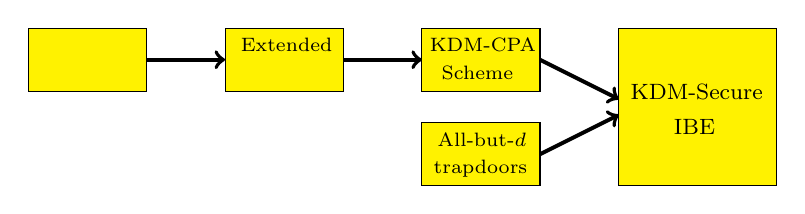
\begin{tikzpicture}
    \onslide<2->{
\filldraw[fill=yellow] (-5cm, 1.20cm) 
       rectangle (-3.5cm, 2.00cm);

\filldraw[fill=yellow] (0cm, 1.20cm) 
       rectangle (1.5cm, 2.00cm);
       \filldraw[fill=yellow] (0cm, 0cm) 
       rectangle (1.5cm, 0.8cm);
       \filldraw[fill=yellow] (-2.5cm,1.20cm)
       rectangle(-1.0cm,2.00cm);
       \filldraw[fill=yellow] (2.5cm, 0cm) 
       rectangle (4.5cm, 2cm);
       \draw[->,line width=0.05cm] (-1.0cm, 1.6cm) -- (0.0cm, 1.6cm);
       \draw[->, line width=0.05cm] (1.5cm, 1.6cm) -- (2.5cm, 1.1cm);
       \draw[->, line width=0.05cm] (1.5cm, 0.4cm) -- (2.5cm, 0.9cm);
       \draw[->, line width=0.05cm] (-3.5cm, 1.6cm) -- (-2.5cm, 1.6cm);
   \pgftext[at=\pgfpoint{-4.5cm}{1.5cm},left,base]{\scriptsize $\mylwe$}
     \pgftext[at=\pgfpoint{0.1cm}{1.70cm},left,base]{\scriptsize KDM-CPA}
    \pgftext[at=\pgfpoint{0.25cm}{1.35cm},left,base]{\scriptsize Scheme}  
    \pgftext[at=\pgfpoint{-2.3cm}{1.7cm},left,base]{\scriptsize Extended}
    \pgftext[at=\pgfpoint{-2.0cm}{1.35cm},left,base]{\scriptsize $\mylwe$}
    \pgftext[at=\pgfpoint{0.2cm}{0.5cm},left,base]{\scriptsize All-but-$d$}
    \pgftext[at=\pgfpoint{0.15cm}{0.15cm},left,base]{\scriptsize trapdoors}
    \pgftext[at=\pgfpoint{3.2cm}{0.65cm},left,base]{\footnotesize IBE}
   \pgftext[at=\pgfpoint{2.65cm}{1.10cm},left,base]{\footnotesize KDM-Secure}

}
      \end{tikzpicture}
    \end{figure}
\end{frame}

\begin{frame}{Learning With Errors (LWE)}
\begin{block}<+->{Definition (Decision Version)}
    
     Given: {\centering
       $(\unif{\matA} \gets \Z_q^{n \times m}, \vecb \gets \Z_q^{m})$}
     \medskip
    
     Distinguish
     $\vecb^t=\short{\vecx_0^{t}}\unif{\matA}+\short{\vecx_1^{t}}$ from
     $\unif{\vecb}$ uniform, where
     $\short{\vecx}=(\short{\vecx_0},\short{\vecx_1})  \Z^{m+n}$\\
     \bigskip
     Distribution for $(\short{\vecx_0}, \short{\vecx_1})$ denoted
     $\chi$, usually  a discrete Gaussian.
    \smallskip
  \end{block}
\begin{itemize}
\item<+-> First defined by Oded Regev~\inlinecite{Regev '05}, who gave a
  quantum reduction from worst-case lattice problems. 
\item<+-> Classical
  reductions have been given in~\inlinecite{P'09, BLPRS'13}
\item<+-> Can easily be seen as the hardness of  decoding a random lattice
\item<+-> The above definition with secret and error from same
  distribution shown
  equivalent to standard LWE in~\inlinecite{ACPS '09}

\end{itemize}
\end{frame}
%%% Local Variables: 
%%% mode: latex
%%% TeX-master: "slides"
%%% End: 
